%!TEX program = xelatex
%# -*- coding: utf-8 -*-
%!TEX encoding = UTF-8 Unicode

\documentclass[12pt,oneside,a4paper]{article}
\usepackage{geometry}
\geometry{verbose,tmargin=2cm,bmargin=2cm,lmargin=2cm,rmargin=2cm}
\usepackage[pdfusetitle,
 bookmarks=true,bookmarksnumbered=true,bookmarksopen=true,bookmarksopenlevel=2,
 breaklinks=false,pdfborder={0 0 1},backref=false,colorlinks=false]
 {hyperref}
\hypersetup{pdfstartview={XYZ null null 1}}
\usepackage{url}
\setcounter{secnumdepth}{2}
\setcounter{tocdepth}{2}
\usepackage{microtype}

\usepackage{amsmath, amsthm, amssymb, amsfonts}
\usepackage[retainorgcmds]{IEEEtrantools}

\usepackage{algorithm}
\usepackage{algorithmic}
\renewcommand{\algorithmicrequire}{\textbf{Input:}} 
\renewcommand{\algorithmicensure}{\textbf{Output:}} 

\usepackage[sc]{mathpazo}
\linespread{1.1}
\usepackage[T1]{fontenc}


\usepackage{graphics}
\usepackage{graphicx}
\usepackage[figure]{hypcap}
\usepackage[hypcap]{caption}
\usepackage{tikz}
%\usepackage{grffile} 
%\usepackage{float} 
\usepackage{pdfpages}

\usepackage{multirow}
\usepackage{booktabs}
\usepackage{threeparttable}

%\usepackage[square,numbers,super,comma,sort]{natbib}
%\usepackage[backend=biber, style=nature, sorting=none, isbn=false, url=false, doi=false]{biblatex}
%\addbibresource{ref.bib}
%\usepackage[]{authblk}

\usepackage{verbatim}
\usepackage{listings}
\usepackage{color}

\newcommand{\problem}[1]
{
    \clearpage
    \section*{Problem {#1}}
}

\newcommand{\subproblem}[1]
{
    \subsection*{Problem {#1}}
}


\newcommand{\solution}
{
    \vspace{15pt}
    \noindent\ignorespaces\textbf{\large Solution}\par
}

\usepackage{fancyhdr}
\usepackage{extramarks}
\lhead{\hmwkAuthorName}
\chead{\hmwkTitle}
\rhead{\firstxmark}
\cfoot{\thepage}

\newcommand{\hmwkTitle}{CSCI 5304 HW 3}
\newcommand{\hmwkAuthorName}{Jingxiang Li}

\setlength\headheight{15pt}
\setlength\parindent{0pt}
\setlength{\parskip}{0.5em}

\newcommand{\m}[1]{\texttt{{#1}}}


\pagestyle{fancy}

\title{\hmwkTitle}
\author{\hmwkAuthorName}
\date{\today}

\begin{document}

\definecolor{mygreen}{rgb}{0,0.6,0}
\definecolor{mygray}{rgb}{0.5,0.5,0.5}
\definecolor{mymauve}{rgb}{0.58,0,0.82}

\lstset{ %
  backgroundcolor=\color{white},   % choose the background color; you must add \usepackage{color} or \usepackage{xcolor}
  basicstyle=\small\ttfamily,        % the size of the fonts that are used for the code
  breakatwhitespace=false,         % sets if automatic breaks should only happen at whitespace
  breaklines=true,                 % sets automatic line breaking
  captionpos=b,                    % sets the caption-position to bottom
  commentstyle=\color{mygreen},    % comment style
  deletekeywords={...},            % if you want to delete keywords from the given language
  escapeinside={\%*}{*)},          % if you want to add LaTeX within your code
  extendedchars=true,              % lets you use non-ASCII characters; for 8-bits encodings only, does not work with UTF-8
  frame=single,                    % adds a frame around the code
  keepspaces=true,                 % keeps spaces in text, useful for keeping indentation of code (possibly needs columns=flexible)
  keywordstyle=\color{blue},       % keyword style
  language=Octave,                 % the language of the code
  morekeywords={*,...},            % if you want to add more keywords to the set
  numbers=left,                    % where to put the line-numbers; possible values are (none, left, right)
  numbersep=10pt,                   % how far the line-numbers are from the code
  numberstyle=\tiny\color{mygray}, % the style that is used for the line-numbers
  rulecolor=\color{black},         % if not set, the frame-color may be changed on line-breaks within not-black text (e.g. comments (green here))
  showspaces=false,                % show spaces everywhere adding particular underscores; it overrides 'showstringspaces'
  showstringspaces=false,          % underline spaces within strings only
  showtabs=false,                  % show tabs within strings adding particular underscores
  stepnumber=1,                    % the step between two line-numbers. If it's 1, each line will be numbered
  stringstyle=\color{mymauve},     % string literal style
  tabsize=2,                       % sets default tabsize to 2 spaces
  title=\lstname,                   % show the filename of files included with \lstinputlisting; also try caption instead of title
  aboveskip=\baselineskip, 
  belowskip=-1 \baselineskip
}


\maketitle


\problem{1}
Consider the matrices $$A = \begin{pmatrix}
  1 & -1 \\
  1 & -1.00001
 \end{pmatrix} \quad B = \begin{pmatrix}
   1 & -1 \\
  -1 & 1.00001
  \end{pmatrix}$$

What is ratio of the largest to smallest eigenvalues (in modulus) for $A$ and for $B$? Show that $k_{2}(A) = k_{2}(B)$. What can you conclude about the ratio of the largest to smallest eigenvalues as a way of estimating sensitivity of a linear system? Would you consider $A$ to be well-conditioned or ill-conditioned?

\solution

First, let's see the ratio of the largest to smallest eigenvalues (in modulus) for $A$ and for $B$.

\begin{lstlisting}
A = [1, -1; 1, -1.00001];
B = [1, -1; -1, 1.00001];
eig_A = eig(A);
eig_B = eig(B);
max(abs(eig_A)) / min(abs(eig_A))
% > 1.0032
max(abs(eig_B)) / min(abs(eig_B))
% > 4.0000e+05
\end{lstlisting}

Note that the ratio for $A$ is $1.0032$, which is much smaller than $B$'s ratio $4.0000e+05$.

Then, we show that $k_{2}(A) = k_{2}(B)$ by using SVD decomposition and \m{Matlab} function \m{cond}.

\begin{lstlisting}
max(svd(A)) / min(svd(A))
% > 4.0000e+05
max(svd(B)) / min(svd(B))
% > 4.0000e+05

cond(A, 2)
% > 4.0000e+05
cond(B, 2)
% > 4.0000e+05
\end{lstlisting}

Note that both SVD and function \m{cond} show that $k_{2}(A) = k_{2}(B)$.

We can conclude that the ratio of the largest to smallest eigenvalues is not a robust way of estimating sensitivity of a linear system. 

Further, I won't consider $A$ to be well-conditioned for the following two reasons: 
\begin{enumerate}
  \item SVD and function \m{cond} show that the condition number of $A$ is very large.
  \item $-1.00001$ is so close to $-1$, and if we see it as $-1$ matrix A become singular, so that A is obviously ill-conditioned.
\end{enumerate}

\problem{2}

\subproblem{a}
Find the $LU$ factorization of the matrix:
$$A = \begin{pmatrix}
2 & 0 & 5 & 8\\
0 & 2 & -1 & -3\\
-2 & 6 & 2 & -3\\
4 & -4 & 0 & 2
\end{pmatrix}$$

\solution
Here we define a function \m{LU\_nopvt} for $LU$ decomposition without partial pivoting for square matrix.

\begin{lstlisting}
%%  LU_nopvt: LU decomposition without partial pivoting using Gaussian Transformation
%%  Input:      A, square matrix recommended
%%  Output:     L U, L is lower-triangular, U is upper-triangular.

function [L U] = LU_nopvt(A)
    
    n = size(A);
    n = n(1);
    
    M = eye(size(A));
    L = eye(size(A));

    for k = 1 : (n - 1)
        gamma = zeros(n, 1);
        for i = (k + 1) : n
            gamma(i) = A(i, k) ./ A(k, k);
        end
        tmp = zeros(n, 1);
        tmp(k) = 1;
        M = eye(n) - gamma * tmp';
        A = M * A;
        L = L * (eye(n) + gamma * tmp');
    end

    U = A;
end
\end{lstlisting}
\clearpage
Then we apply function \m{LU\_nopvt} to matrix $A$.

\begin{lstlisting}
A = [2, 0, 5, 8; 0, 2, -1, -3; -2, 6, 2, -3; 4, -4, 0, 2];
[L U] = LU_nopvt(A);

L
% >  1.0000         0         0         0
% >  0         1.0000         0         0
% > -1.0000    3.0000    1.0000         0
% >  2.0000   -2.0000   -1.2000    1.0000

U
% >  2.0000         0    5.0000    8.0000
% >       0    2.0000   -1.0000   -3.0000
% >       0         0   10.0000   14.0000
% >       0         0         0   -3.2000
\end{lstlisting}

\subproblem{b}
Find the $PA=LU$ factorization of $A$ using partial pivoting.

\solution
\begin{lstlisting}
[L,U,P] = lu(A);

L
% >  1.0000         0         0         0
% > -0.5000    1.0000         0         0
% >  0.5000    0.5000    1.0000         0
% >  0         0.5000   -0.5000    1.0000

U
% > 4    -4     0     2
% > 0     4     2    -2
% > 0     0     4     8
% > 0     0     0     2

P
% > 0     0     0     1
% > 0     0     1     0
% > 1     0     0     0
% > 0     1     0     0
\end{lstlisting}

\subproblem{c}
What is the determinant of $A$?

\solution
Given $PA = LU$, we have $$det(A) = \frac{det(L)det(U)}{det(P)}$$
it's easy to see that $det(L) = 1$, $det(U) = \prod_{i = 1}^{4}{U_{ii}} = 128$, $det(P) = -1$, so that $$det(A) = 128 / -1 = -128$$

\subproblem{d}
Using the $LU$ factors obtained in (a) find the second column of the inverse of $A$, without computing the whole inverse.

\solution
Note that
$$A^{-1} \cdot (0, 1, 0, 0)^{T} = A^{-1}_{2}$$
then let $x = A^{-1}_{2}$, $b = (0, 1, 0, 0)^{T}$, We have 
$Ax = b$, i.e. $LUx = b$. To obtain x, we first solve $Ly = b$, then $Ux = y$. 

We first define two functions \m{Forw\_sub} and \m{Back\_sub} for forward substitution and backward substitution.

\begin{lstlisting}
%%  Back_sub: Backward substitution to solve Ax = b where A is upper-triangular
%%  Input: A, b
%%  Output: x
function [x] = Back_sub(A, b)
    n = length(b);
    foo = 0;

    for i = n : -1 : 2
        for j = (i - 1) : -1 : 1
            foo = A(j, i) ./ A(i, i);
            A(j, :) = A(j, :) - foo * A(i, :);
            b(j) = b(j) - foo * b(i);
        end
    end

    x = b ./ diag(A);
end
\end{lstlisting}

\begin{lstlisting}
%%  Forw_sub: Forward substitution to solve Ax = b where A is lower-triangular
%%  Input: A, b
%%  Output: x
function [x] = Forw_sub(A, b)    
    n = length(b);
    foo = 0;

    for i = 1 : (n - 1)
        for j = (i + 1) : n
            foo = A(j, i) ./ A(i, i);
            A(j, :) = A(j, :) - foo * A(i, :);
            b(j) = b(j) - foo * b(i);
        end
    end

    x = b ./ diag(A);    
end
\end{lstlisting}

Then we apply \m{Forw\_sub} and \m{Back\_sub} to the $LU$ decomposition result, to obtain the second column of the inverse of $A$.

\begin{lstlisting}
[L U] = LU_nopvt(A);
b = [0, 1, 0 ,0]';
y = Forw_sub(L, b);
x = Back_sub(U, y);

x
% >  0.5000
% >  0.7500
% > -1.0000
% >  0.5000
\end{lstlisting}

\problem{3}

\subproblem{a}
Show that if $A$ is Symmetric Positive Definite (SPD) then $Trace(AX) > 0$ for all SPD matrices $X$.

\solution
We calculate Cholesky decomposition for $A$ and $X$, say $A = L_{A}L_{A}^{T}$, $X = L_{X}L_{X}^{T}$, then
$$Trace(AX) = Trace(L_{A}L_{A}^{T}L_{X}L_{X}^{T}) = Trace(L_{A}^{T}L_{X}L_{X}^{T}L_{A})$$
let $M = L_{A}^{T}L_{X}$, then 
$$Trace(AX) = Trace(MM^{T})$$
Let $M = (M_{1}, M_{2}, M_{3}, M_{4})^{T}$, then 
$$Trace(MM^{T}) = \sum_{i = 1}^{4}(||M_{1}||_{2}^{2}) > 0 $$
Q.E.D.

\subproblem{b}
Show that if $Trace(AX) \geq 0$ for all Symmetric Positive Semi-Definite (PSD) matrices $X$ then $A$ is PSD.

\solution
We first decompose $X = LL^{T}$, then
$$Trace(AX) = Trace(ALL^{T}) = Trace(L^{T}AL)$$
$L$ is a lower-triangular matrix, Let $L = (L_{1},\dots,L_{n})$. Then
$$Trace(AX) = L_{1}^{T}AL_{1} + L_{2}^{T}AL_{2} + \dots + L_{3}^{T}AL_{3} \geq 0$$
We will then prove it by contradiction. Suppose A is not PSD, then $\exists x~~s.t.~~x^{T}Ax < 0$. then we can construct $L^{*} = (x, 0, 0, \dots)$ and let $X^{*} = L^{*}{L^{*}}^{T}$, then $Trace(AX^{*}) =  x^{T}Ax < 0$, contradiction. So that A is PSD.\par Q.E.D.

\problem{4}
Write Matlab functions to carry out Gaussian Elimination without pivoting to solve a linear system $Ax = b$ where $A$ is a tridiagonal matrix, stored as three columns (the subdiagonal, the main diagonal, and the superdiagonal), and $b$ is a vector of all ones of appropriate dimension. You’ll need to write at least two functions, one to carry out Gaussian Elimination on A, together with $b$, and one to solve the resulting triangular system.

Your matlab function should avoid storing the matrix as a full matrix or sparse matrix, though you can use one of these to check your answers with the Matlab built in functions. Apply this function to the matrix formed by the following Matlab expression:

\begin{verbatim}
m = 10 or 500 or something bigger;
A_trid = [ [nan; ones(2*m,1)*m ], (m+1+(-m:m)') , [ones(2*m,1)*m;nan]];
% the following converts the tridiagonal to a full matrix
% (just for the purpose of checking your answers)
A_full = diag(A_trid(:,2))+diag(A_trid(2:end,1),-1)+diag(A_trid(1:end-1,3),1);
\end{verbatim}

The right hand side for this will be a vector of all ones of dimension $n = 2m + 1$, $e_{n}$.

Do all this for $m = 500 : 500 : 5000$ and time the elapsed time or CPU time for solving the linear system. To time the process, you can use the Matlab functions tic, toc, etime, or cputime. Submit a table of CPU or elapsed times together with norms of the residuals. What seems to be the complexity of solving tridiagonal linear systems? Is it $O(n)$, $O(n^2)$ or $O(n^3)$? Optionally, solve the linear systems with Matlab explicitly and compare the accuracy and costs of the two different solutions. Are they close or not?

\solution
We first define two functions \m{GE\_Band} and \m{UpTri\_Band}. \m{GE\_Band} is designed for carrying out Gaussian Elimination on a tridiagonal matrix $A$ stored as $n\times 3$, together with $b$. \m{UpTri\_Band} is the backward substitution algorithm to solve the linear system $Ax = b$. (Note that we call function \m{UpTri\_Band} at the end of \m{GE\_Band}, so that the return value for \m{GE\_Band} will directly be the solution $x$). The following code chunk will contain these two functions.

\begin{lstlisting}
%% GE-Band: Gaussian Elimination without pivoting for tridiagonal matrix stored as n * 3
%% Input  A: tridiagonal matrix stored as n * 3
%%      b: n-dimensional vector
%% outputs  x: the solution for system Ax = b

function [x] = GE_Band(A, b)

    n = size(b); %% number of rows
    multiplier = 0; %% multiplier used in each step of GE

    %% for loop for Gaussian Elimination
    for i = 1 : (n - 1)
        multiplier = A(i + 1, 1) / A(i, 2);
        A(i + 1, :) = A(i + 1, :) - [A(i, 2 : 3), 0] * multiplier;
        b(i + 1) = b(i + 1) - b(i) * multiplier;
    endfor
    
    %% Call function to solve the upper triangle linear system
    x = UpTri_Band(A, b);

end


%% UpTri_Band: Solve a linear system Ax = b, 
%% where A is an upper triangle matrix stored as n * 3 (obtained from GE_Band)
%% Input:   A, b from GE_Band
%% Output:  x, solution to the linear system

function [x] = UpTri_Band(A, b)

    n = size(b); %% size of b
    multiplier = 0; %% multiplier used in loop

    for i = (n - 1) : (-1) : 1
        multiplier = A(i, 3) / A(i + 1, 2);
        A(i, :) = A(i, :) - multiplier .* [0, A(i + 1, 1 : 2)];
        b(i) = b(i) - multiplier * b(i + 1);
    endfor

    x = b ./ A(:, 2);

end
\end{lstlisting}

Then we can verify our functions by comparing them with the built-in Matlab function for full matrix given a small $m$.

\begin{lstlisting}
%% verify our functions by comparing GE_Band with Matlab built-in fucntions when m = 3

m = 3;
A_trid = [ [nan; ones(2*m,1)*m ], (m+1+(-m:m)') , [ones(2*m,1)*m;nan]];
A_full = diag(A_trid(:,2))+diag(A_trid(2:end,1),-1)+diag(A_trid(1:end-1,3),1);
b = ones(size(A_trid, 1), 1);

[GE_Band(A_trid, b) inv(A_full) * b]
% > -0.15116  -0.15116
% >  0.38372   0.38372
% >  0.22868   0.22868
% > -0.27907  -0.27907
% >  0.47674   0.47674
% > -0.18217  -0.18217
% >  0.22093   0.22093
\end{lstlisting}

It shows that the solution given by our functions is exactly the same as the solution given by the Matlab's built-in function, indicating that our functions work well in solving linear system with tridiagonal matrix.

Then we will test the functions for $m = 500 : 500 : 5000$, and report the elapsed time for each $m$ together with norms of the residuals.

\begin{lstlisting}
%% test the functions for m = 500 : 500 : 5000, and report the elapsed time and norms of the residuals

m_array = 500 : 500 : 5000;
result_time = zeros(size(m_array)(2), 1);
result_res = zeros(size(m_array)(2), 1);
for i = 1 : size(m_array)(2)
    m = m_array(i);
    A_trid = [ [nan; ones(2*m,1)*m ], (m+1+(-m:m)') , [ones(2*m,1)*m;nan]];
    A_full = diag(A_trid(:,2))+diag(A_trid(2:end,1),-1)+diag(A_trid(1:end-1,3),1);
    b = ones(size(A_trid, 1), 1);
    tic();
        x1 = GE_Band(A_trid, b);
        % x1 = A_full \ b;
    result_time(i) = toc();
    result_res(i) = norm(b - A_full * x1, 1);
endfor

[result_time, result_res]
% > 7.8816e-02   1.6211e-12
% > 1.5276e-01   7.7149e-13
% > 2.3571e-01   3.8237e-12
% > 3.0822e-01   1.0439e-12
% > 3.8363e-01   2.6795e-12
% > 4.7035e-01   6.9070e-12
% > 5.7751e-01   4.3037e-12
% > 6.1196e-01   2.8538e-12
% > 6.8640e-01   4.1214e-12
% > 7.6434e-01   3.4363e-12
\end{lstlisting}

The resulting elapsed time and norms of residuals are reported above. \clearpage

To see the complexity of solving tridiagonal linear system, we can plot a line chart for the elapsed time against $m$. As we can see in figure \ref{scenA}, there is an obvious linear relationship between elapsed time and $m$, suggesting that the complexity of solving tridiagonal linear systems is $O(n)$

\begin{figure}[!ht]
  \centering
  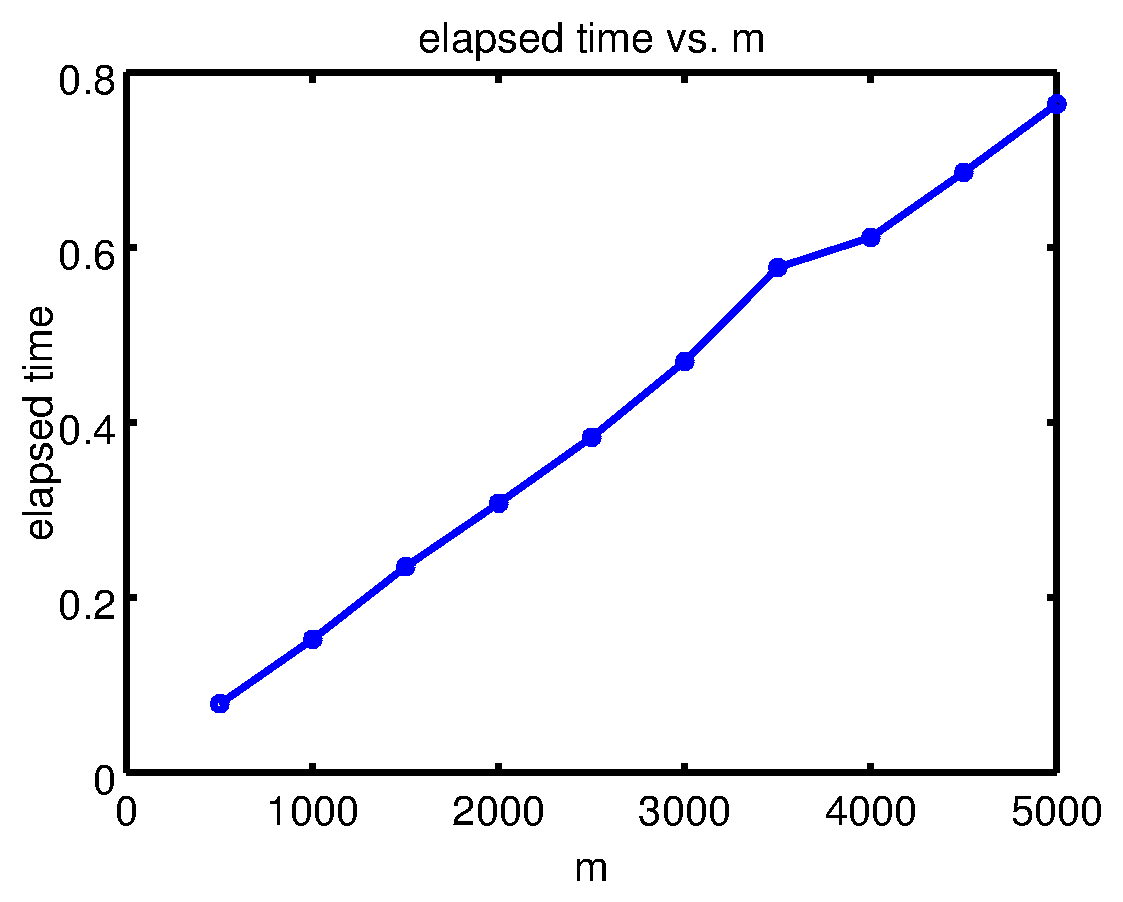
\includegraphics[scale=0.6]{./Graph/time_vs_m.pdf}
  \caption{elapsed time vs. m}
  \label{scenA}
\end{figure}

Then we compare our functions with the Matlab built-in functions. 

\begin{lstlisting}
%% Compare our functions with Matlab to show the superiority of our functions.

m_array = 500 : 250 : 2500;
result_time = zeros(size(m_array)(2), 2);
result_res = zeros(size(m_array)(2), 2);
for i = 1 : size(m_array)(2)
    m = m_array(i);
    A_trid = [ [nan; ones(2*m,1)*m ], (m+1+(-m:m)') , [ones(2*m,1)*m;nan]];
    A_full = diag(A_trid(:,2))+diag(A_trid(2:end,1),-1)+diag(A_trid(1:end-1,3),1);
    b = ones(size(A_trid, 1), 1);
    tic();
        x1 = GE_Band(A_trid, b);
    result_time(i, 1) = toc();
    result_res(i, 1) = norm(b - A_full * x1, 1);
    tic();
      x2 = A_full \ b;
    result_time(i, 2) = toc();
    result_res(i, 2) = norm(b - A_full * x2, 1);
endfor

[result_time result_res]
% > 7.6898e-02   1.0637e-01   1.6211e-12   1.9318e-14
% > 1.0888e-01   2.9426e-01   3.7359e-13   3.5971e-14
% > 1.5138e-01   7.2223e-01   7.7149e-13   5.1292e-14
% > 1.8058e-01   1.2491e+00   1.2113e-12   1.6820e-13
% > 2.1552e-01   2.0951e+00   3.8237e-12   5.5300e-13
% > 2.5187e-01   3.2953e+00   2.3949e-12   1.0525e-13
% > 2.8727e-01   4.8834e+00   1.0439e-12   8.1157e-14
% > 3.2394e-01   6.8370e+00   1.0638e-12   8.9595e-14
% > 3.7854e-01   9.3374e+00   2.6795e-12   1.2967e-13
\end{lstlisting}

Note that the backward error of Matlab's built-in function is only slightly better than our function's. However, our functions dominate Matlab in terms of the elapsed time. 

\problem{5}
Write a Matlab code that computes the $QR$ factorization of a tridiagonal matrix $A$ stored in the same compact form as given in the previous question, to solve the same system $Ax = b$ with $b$ as before as well. The result should be $QR = A$, with $R$ stored in the similar compact form as $A$ (need additional space for one extra superdiagonal), and $Q$ should be left as a sequence of Givens rotations or $2 \times 2$ Householder transformations. You can apply the Givens rotations or reflections to $b$ as you go, to obtain $Q^{T}b$, and then solve the triangular system $Rx = Q^{T}b$ with a triangular system solver similar to that used in the previous question. In this case, the upper triangular will have two non-zero diagonals above the main diagonal, instead of just one.

Each Givens rotation of the form is specified by the two numbers $c$, $s$ and the indices of the rows they apply to, where $c^2 + s^2 = 1$. In this problem, the first Givens rotation is between rows 1 and 2, so the Givens rotation could be stored in compact form as a row vector $[c, s, 1, 2]$. The entire $Q$ is then stored as a stack of $n − 1$ such row vectors. To check your answers, you would need to write a function to multiply out these Givens rotations to form the explicit $Q$ to compare with the output from Matlab’s built-in $qr$ function.

\solution
Here we define three functions: \m{Given\_trans}, \m{QR\_Given} and \m{UpTri\_Band4}. \m{Given\_trans} is to do Given transformation given $x_{i}$, $x_{j}$, $c$ and $s$; \m{QR\_Given} is to do $QR$ decomposition on a tridiagonal matrix $A$, together with $b$, the output of \m{QR\_Given} will be $R$ and $Q^{T}b$; \m{UpTri\_Band4} is the backward substitution algorithm.

\begin{lstlisting}
%% Calculate Given Transformation
%% Input x1, x2, c, s
%% Output tmp1, tmp2 (transformed x1 and x2)

function [tmp1 tmp2] = Given_trans(x1, x2, c, s)
    tmp1 = c * x1 - s * x2;
    tmp2 = s * x1 + c * x2;
end


%% QR_Given: Solve Ax = b, where A is a tridiagonal matrix stored as n * 3
%% Using Given Rotation
%% Input:   A, n * 3
%%          b, n * 1
%% Output:  A = R and b = Q' * b, 
%%          s.t. A * x = b
%%          Q, stored as [c, s, i, j]

function [A b Q] = QR_Given(A, b)

    n = size(b)(1);
    A = [A, zeros(n, 1)];
    A((n - 1) : n, 4) = NaN;
    Q = zeros(n - 1, 4);

    for i = 1 : (n - 1)
        j = i + 1;
        xi = A(i, 2);
        xj = A(j, 1);
        c = xi / sqrt(xi^2 + xj^2);
        s = -xj / sqrt(xi^2 + xj^2);
        A(i, 2) = c * xi - s * xj;
        A(j, 1) = s * xi + c * xj;
        [tmp1 tmp2] = Given_trans(A(i, 3), A(j, 2), c, s);
        A(i, 3) = tmp1;
        A(j, 2) = tmp2;
        if (j < n)
            [tmp1 tmp2] = Given_trans(A(i, 4), A(j, 3), c, s);
            A(i, 4) = tmp1;
            A(j, 3) = tmp2;
        end
        bi = b(i);
        bj = b(j);
        b(i) = c * bi - s * bj;
        b(j) = s * bi + c * bj;
        Q(i, :) = [c, s, i, j];
    end

end


%% UpTri_Band4: Solve a linear system Ax = b, 
%% where A is an upper triangle matrix stored as n * 4
%% Input:   A, b from QR_Given
%% Output:  x, solution to the linear system

function [x] = UpTri_Band4(A, b)

    n = size(b); %% size of b
    multiplier = 0; %% multiplier used in loop

    for i = (n - 1) : (-1) : 1
        multiplier = A(i, 3) / A(i + 1, 2);
        A(i, :) = A(i, :) - multiplier .* [0, A(i + 1, 1 : 3)];
        b(i) = b(i) - multiplier * b(i + 1);
        if (i > 1)
          multiplier = A(i - 1, 4) / A(i + 1, 2);
          A(i - 1, :) = A(i - 1, :) - multiplier .* [0, 0, A(i + 1, 1 : 2)];
          b(i - 1) = b(i - 1) - multiplier * b(i + 1);
        end 
        
    endfor

    x = b ./ A(:, 2);

end
\end{lstlisting} 

Then we can verify our functions by comparing them with Matlab's built-in functions for a very small m.

\begin{lstlisting}
%% verify our functions by comparing them with Matlab built-in fucntions when m = 3

m = 3;
A_trid = [ [nan; ones(2*m,1)*m ], (m+1+(-m:m)') , [ones(2*m,1)*m;nan]];
A_full = diag(A_trid(:,2))+diag(A_trid(2:end,1),-1)+diag(A_trid(1:end-1,3),1);
b = ones(size(A_trid, 1), 1);

[R b1] = QR_Given(A_trid, b);
x = UpTri_Band4(R, b1);

[A_full \ b x]
% > -0.15116  -0.15116
% >  0.38372   0.38372
% >  0.22868   0.22868
% > -0.27907  -0.27907
% >  0.47674   0.47674
% > -0.18217  -0.18217
% >  0.22093   0.22093
\end{lstlisting}

Note that the solution given by our functions is exactly the same as the one given by Matlab's built-in function, suggesting that our functions are correct.

Next, we will claim function \m{Q\_trans} that can transform $Q$ from a stack of $[c, s, 1, 2]$ to the explicit matrix $Q$, and then we will compare this $Q$ with the one obtained from \m{qr} function in Matlab.

\begin{lstlisting}
%% Q_trans Transform Q from [c, s, i, j] to matrix
%% Input    Q from QR_Given
%%          n size of Given transformation matrix
%% functionname: function description

function [Q1] = Q_trans(Q, n)

    Q1 = eye(n);

    for k = 1 : size(Q, 1)
        c = Q(k, 1);
        s = Q(k, 2);
        i = Q(k, 3);
        j = Q(k, 4);
        tmp = eye(n);
        tmp(i, i) = c;
        tmp(j, j) = c;
        tmp(i, j) = s;
        tmp(j, i) = -s;
        Q1 = Q1 * tmp;
    end

end
\end{lstlisting}

Now we compare $Q$ from \m{QR\_Given\_Q} with $Q$ from \m{qr}, with m = 3;

\begin{lstlisting}
%% Compare Q from QR_Given_Q with Q1 from qr when m = 2

m = 2;
A_trid = [ [nan; ones(2*m,1)*m ], (m+1+(-m:m)') , [ones(2*m,1)*m;nan]];
A_full = diag(A_trid(:,2))+diag(A_trid(2:end,1),-1)+diag(A_trid(1:end-1,3),1);
b = ones(size(A_trid, 1), 1);

n = size(A_trid, 1);
[R b1 Q] = QR_Given(A_trid, b);
Q = Q_trans(Q, n);
[Q1 R1] = qr(A_full);

Q
% > 0.44721   0.36515  -0.58321   0.43004   0.37629
% > 0.89443  -0.18257   0.29161  -0.21502  -0.18814
% > 0.00000   0.91287   0.29161  -0.21502  -0.18814
% > 0.00000   0.00000   0.69985   0.53755   0.47036
% > 0.00000   0.00000   0.00000   0.65850  -0.75258

Q1
% > -0.44721   0.36515   0.58321  -0.43004  -0.37629
% > -0.89443  -0.18257  -0.29161   0.21502   0.18814
% > -0.00000   0.91287  -0.29161   0.21502   0.18814
% > -0.00000   0.00000  -0.69985  -0.53755  -0.47036
% > -0.00000   0.00000  -0.00000  -0.65850   0.75258
\end{lstlisting}

$Q$ above is the orthonormal matrix given by our function, and $Q1$ is the orthonormal matrix obtained from Matlab's \m{qr}. Note that the only difference between $Q$ and $Q1$ is the sign of each column, but that doesn't matter. The result suggests that our functions work well.
\end{document}